\documentclass[10pt]{article}
\usepackage[english]{babel}
\usepackage{url}
\usepackage{graphicx}
\usepackage{lscape}
\usepackage{float}
\usepackage{hyperref}
\usepackage{rotating}
\usepackage{listings}
\usepackage{multirow}
\usepackage{todonotes}
\usepackage{verbatim}
\usepackage{cite}
\usepackage{graphicx}
\usepackage{tabularx}  
\usepackage{array}

\usepackage{listings}
\usepackage{color}

\definecolor{dkgreen}{rgb}{0,0.6,0}
\definecolor{gray}{rgb}{0.5,0.5,0.5}
\definecolor{mauve}{rgb}{0.58,0,0.82}

\lstset{frame=tb,
  language=SQL,
  aboveskip=3mm,
  belowskip=3mm,
  showstringspaces=false,
  columns=flexible,
  basicstyle={\small\ttfamily},
  numbers=none,
  numberstyle=\tiny\color{gray},
  keywordstyle=\color{blue},
  commentstyle=\color{dkgreen},
  stringstyle=\color{mauve},
  breaklines=true,
  breakatwhitespace=true,
  tabsize=3
}

\graphicspath{ {./figures/} }

\usepackage[a4paper, left=3.5cm, right=3.5cm, top=4cm, bottom=3cm]{geometry}

\makeatletter
\renewcommand\paragraph{\@startsection{paragraph}{4}{\z@}%
            {-2ex\@plus -1ex \@minus -.25ex}%
            {1.ex \@plus .25ex}%
            {\normalfont\normalsize\bfseries}}
\makeatother
\setcounter{secnumdepth}{4} 
\setcounter{tocdepth}{4}   

\begin{document}

% HEADER PAGE
\begin{titlepage}
   \begin{center}
       \vspace*{1cm}
       {\fontsize{17}{16}\selectfont\textbf{Model-Driven Software Engineering Assignment}}

       \vspace{0.5cm}
        Model-Driven Software Engineering
            
       \vspace{1.5cm}

       \textbf{Group 2}\\
       \textbf{Fábio Araújo de Sá (up202007658@up.pt)}\\
       \textbf{Filipe Rodrigues Fonseca (up202003474@up.pt)}\\
       \textbf{Lourenço Alexandre Correia Gonçalves (up202004816@up.pt)}\\
       \textbf{Pedro Pereira Ferreira (up202004986@up.pt)}\\
       \vfill
            
       
\includegraphics[width=0.6\textwidth]{imgs/FEUP.png}
        
       \vspace{2cm}
            
       November 2024
            
   \end{center}
\end{titlepage}

\tableofcontents
\clearpage

\section{Introduction}

This project aims to explore techniques and technologies of Model-Driven Software Engineering (MDSE), which can be applied to automate parts of the development of applications on low-code platforms \cite{brambilla2017mdse}. These platforms seek to simplify development by allowing the creation of complex solutions without the need for direct programming.

Throughout this project, we explored the different phases of constructing a pipeline that enables the transformation of ER Models into SQL code. To achieve this, we designed and implemented metamodels representing both ER models and Relational models, and these were validated through specific test cases. Afterward, constraints for the model-to-model transformation were created. Finally, a model-to-text transformation was performed to obtain valid and executable SQL code derived from the initial model.

At every stage, the main challenges were identified, and the decisions made were justified.

\section{Tools and Technologies}

For the implementation of the project, we used the following tools and technologies:

\begin{itemize}

    \item \textbf{Eclipse\footnote{https://www.eclipse.org}}: an integrated development environment (IDE) that served as the main platform for development and the integration of other tools;
    
    \item \textbf{Ecore\footnote{https://wiki.eclipse.org/Ecore/}}: part of the Eclipse Modeling Framework (EMF), which allows the creation, manipulation, and validation of metamodels. It was used to define the formal languages for the source and target models;

    \item \textbf{XMI\footnote{https://www.omg.org/spec/XMI/}}: XML Metadata Interchange, is a standard for exchanging metadata information via Extensible Markup Language.

    \item \textbf{Object Constraint Language (OCL)\footnote{https://projects.eclipse.org/projects/modeling.mdt.ocl}}: used to define integrity constraints on metamodel instances, ensuring that the models adhere to all the necessary rules and consistencies during transformations;
    
    \item \textbf{OCLinEcore\footnote{https://wiki.eclipse.org/OCL/OCLinEcore}}: is an extension that integrates OCL expressions into Ecore models, allowing for more expressive constraints and operations within models;
    
    \item \textbf{Atlas Transformation Language (ATL)\footnote{https://eclipse.dev/atl/}}: used for applying model-to-model (M2M) transformations, enabling the conversion of more abstract models (such as ER models) to domain-specific models (such as relational models);
    
    \item \textbf{Acceleo\footnote{https://projects.eclipse.org/projects/modeling.acceleo}}: a tool for applying model-to-text (M2T) transformations, used to generate code from the final models, allowing, in this case, the generation of valid SQL code;

    \item \textbf{Model Transformation Language (MTL)\footnote{https://eclipse.dev/modeling/transformation.php}}: the Acceleo language to generate code from the target model.
    
\end{itemize}

These tools enabled the automation of the pipeline developed from the proposed models and domains. The use of metamodeling stategies ensured the validation of the models, their transformation, and the appropriate output.

\section{Modeling Domain Analysis}

At this stage, we analyzed the domain to define the source and target models that will be used throughout the project. The analysis of one concrete example helped to delineate the scope of the project, ensuring that our metamodels capture all the concepts covered in the domain and validate each one appropriately.

\subsection{Domain}

To understand the domain and define the project's boundaries, we analyzed practical one example of two types of models commonly used as the foundation for generating SQL code: Entity-Relationship (ER) models and Relational models. This example guided the development of the metamodels and also served as test cases in the subsequent phases.

\subsubsection{ER Model}

The Entity-Relationship (ER) model\footnote{https://en.wikipedia.org/wiki/Entity–relationship-model}\footnote{https://www.geeksforgeeks.org/introduction-of-er-model/} is a conceptual approach to data modeling that visually represents the logical structure of an information system and the relationships between the data within that system. Taking the concrete example of a chain of gyms with equipment, where each gym can have multiple customers, and them can have some characteristics in the system, we can derive the ER model as represented in Figure \ref{figure1}:

\begin{center}
    \begin{figure}[H]
        \centering
        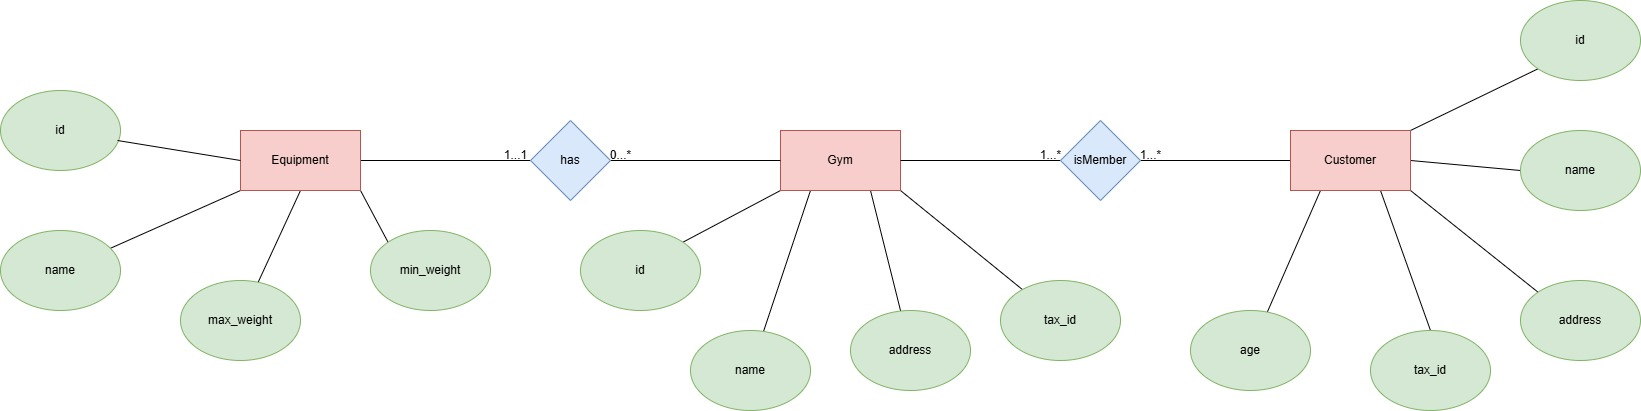
\includegraphics[width=1.0\textwidth]{imgs/er-model.png}
            \caption{Gym ER Model example}
        \label{figure1}
    \end{figure}
\end{center}

In this example, as well as in similar models, it is essential to ensure the existence of:

\begin{itemize}
    \item Entities;
    \item Attributes with associated entities;
    \item Relationships with various multiplicities (one-to-one, one-to-many, many-to-many) between entities.
\end{itemize}

For the sake of simplifying future validations, the system will only be designed to handle attributes of type string and integer. Thus, the model is considered valid if it allows the creation of attributes with these types, entities with attributes, and relationships of any cardinality between the entities in the system.

\subsubsection{Relational Model}

The Relational Model\footnote{https://www.geeksforgeeks.org/relational-model-in-dbms/} is a data modeling approach that organizes information into tables, or relations, where each table consists of columns (its attributes) and rows (the actual data). Unlike the Entity-Relationship (ER) model, which is more conceptual and visual, the relational model focuses on the effective implementation of data in Database Management Systems (DBMS), thereby aligning more closely with the ultimate goal of generating SQL code. Using the previous example of the chain of gyms, a translation of the above into a Relational Model can be represented as shown in Figure \ref{figure2}:

\begin{center}
    \begin{figure}[H]
        \centering
        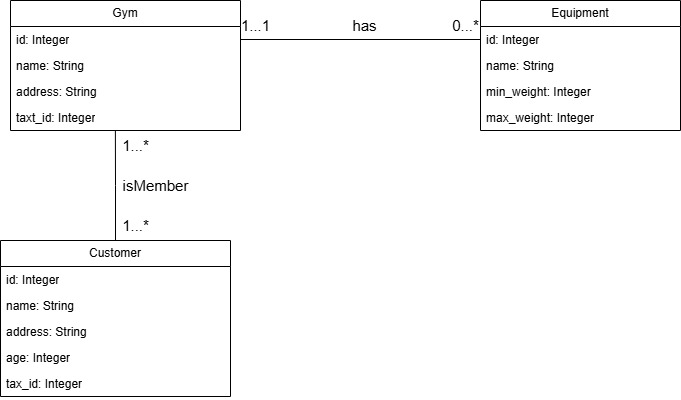
\includegraphics[width=0.9\textwidth]{imgs/relational-model.png}
            \caption{Gym Relational Model example}
        \label{figure2}
    \end{figure}
\end{center}

Thus, the relational models to be manipulated will include:

\begin{itemize}

    \item Varied multiplicities between tables (one-to-one, one-to-many, many-to-many);
    
    \item Tables with multiple attributes, including the necessary primary and foreign keys;
    
    \item Relationships between tables, with the corresponding keys and associated multiplicities.
    
\end{itemize}

In the project, generalizations between tables, self-dependencies, and composite foreign keys were not considered. Any model with these functionalities in our project must be invalidated in the corresponding metamodel.

\subsubsection{SQL Code}

The final objective of the project is to ensure a standard, valid Structured Query Language (SQL) code that can be executed, for example, in one database engine like PostgreSQL\footnote{https://www.postgresql.org}, SQLite3\footnote{https://www.sqlite.org} or MySQL\footnote{https://www.mysql.com}. For the final code to be considered valid, the following requirements must be met:

\begin{itemize}

    \item The output file must have the \textbf{.sql} extension;
    
    \item There must be a schema definition, \textbf{CREATE SCHEMA}, in the file header;
    
    \item There must be \textbf{DROP TABLE} statements in the header of the file to ensure the database can be reset without key collisions or duplicate IDs;
    
    \item The definition of each table, attributes and relationships;
    
    \item The explanation of primary keys and foreign keys, if available.
    
\end{itemize}

The code snippet in Annex \ref{Annex1} demonstrates the expected result from the gym example. It is important to note that in SQL, all generated tables explicitly define their primary keys and, where applicable, the corresponding foreign keys. For standardization purposes, and since not all database engines operate with the same keywords, implementations of internal primary keys using keywords such as \textbf{AUTOINCREMENT}, \textbf{ROWID} or \textbf{SERIAL} have been excluded. Instead, it is assumed that all keys are inserted manually. Conversely, to ensure final code validation in database engines, the \textbf{NOT NULL} constraint should be applied to all primary and foreign key declarations.

\subsection{Concepts}

After defining the problem domain and to gain a more high-level perspective for preparing the corresponding metamodels, the key concepts of both models were gathered and explored.

In the case of the ER model, the following components were identified:

\begin{itemize}

    \item \textbf{Entity}: represents a distinct object or concept within the system;
    
    \item \textbf{Attribute}: defines the characteristics of an entity;
    
    \item \textbf{Relation}: represents the connections between two or more entities.
    
\end{itemize}

Regarding constraints, it is important to note that each entity can have multiple attributes, and each attribute belongs to only one entity. On the other hand, a relation is the result of the connection between a pair of entities. The multiplicity of each relation can be one-to-one, one-to-many, or many-to-many.

In contrast to the previous model, the Relational Model includes other concepts that are more closely aligned with the properties found in SQL:

\begin{itemize}

    \item \textbf{Table}: corresponds to the entity in the previous model;
    
    \item \textbf{Column}: corresponds to the attribute of each entity;
    
    \item \textbf{Primary Key}: column that uniquely identifies each record in the table;
    
    \item \textbf{Foreign Key}: column in a table that references another existent table.
    
\end{itemize}

In terms of constraints, we can conclude that a table in this Relational Model has columns, and each column belongs to a single table. Additionally, there is only one primary key per table, but multiple foreign keys can exist, provided they have a valid reference to another table.

Each of these identified components, along with their constraints, was implemented using Ecore classes. In the following section, we will express the process of creating the corresponding Metamodels.

\section{Metamodel Design}

Having established the key components and constraints of both the Entity-Relationship model and the Relational model, we were ready to delve into the design of the metamodels. Using Ecore, we defined the classes and relationships that encapsulate the identified components, ensuring that they adhere to the constraints we had outlined.

\subsection{ER Metamodel}

The ER Metamodel was formed by:

\begin{itemize}

    \item \textbf{Entity}: has a ename (EString) and can be associated with multiple Attributes;
    
    \item \textbf{Attribute}: has a aname (EString), a data type (EString), isIdentifier (EBoolean) and a correspondent Entity;
    
    \item \textbf{Relation}: has a unique rname (EString) and a multiplicity, defined by two integer pairs (EInt) representing the lower and upper bounds, which describe the number of instances of each entity that can participate in the relationship.
    
\end{itemize}

For many-to-many multiplicity cases, we considered the standard Ecore value: -1. To ensure Ecore compatibility, we added an \textbf{Model} component that can contain all entities and relationships in the system and has a name (EString). Since ER models do not inherently indicate the potential primary keys of entities, and this information is crucial for defining the future relational model, we chose to add a boolean attribute, \textbf{isIdentifier}, which marks attributes that, being unique and non-null, can independently identify the entity within the system.

The Ecore framework generated a visual representation of the metamodel. The Figure \ref{figure3} provides an overview of how entities, attributes, and relations are interconnected:

\begin{center}
    \begin{figure}[H]
        \centering
        
\includegraphics[width=1.0\textwidth]{imgs/er-metamodel.jpeg}
            \caption{ER Metamodel}
        \label{figure3}
    \end{figure}
\end{center}

\subsection{Relational Metamodel}

The Relational Metamodel was formed by:

\begin{itemize}

    \item \textbf{Schema}: has a name (EString) and can be associated with all system Tables;
 
    \item \textbf{Table}: has a name (EString) and can be associated with multiple Columns;
    
    \item \textbf{Column}: has a name (EString), a data type (EString), isNullable (EBoolean), isUnique (EBoolean), and has a correspondent Table;
    
    \item \textbf{Primary Key}: a column that uniquely identifies each record in the table;
    
    \item \textbf{Foreign Key}: a column in one table that creates a link to the primary key of another table, establishing a relationship between the two tables.
    
\end{itemize}

The Ecore framework generates a visual representation of the Relational metamodel, illustrating the relationships between tables, columns, and keys. The Figure \ref{figure4} clarifies how the components interact within the relational structure:

\begin{center}
    \begin{figure}[H]
        \centering
        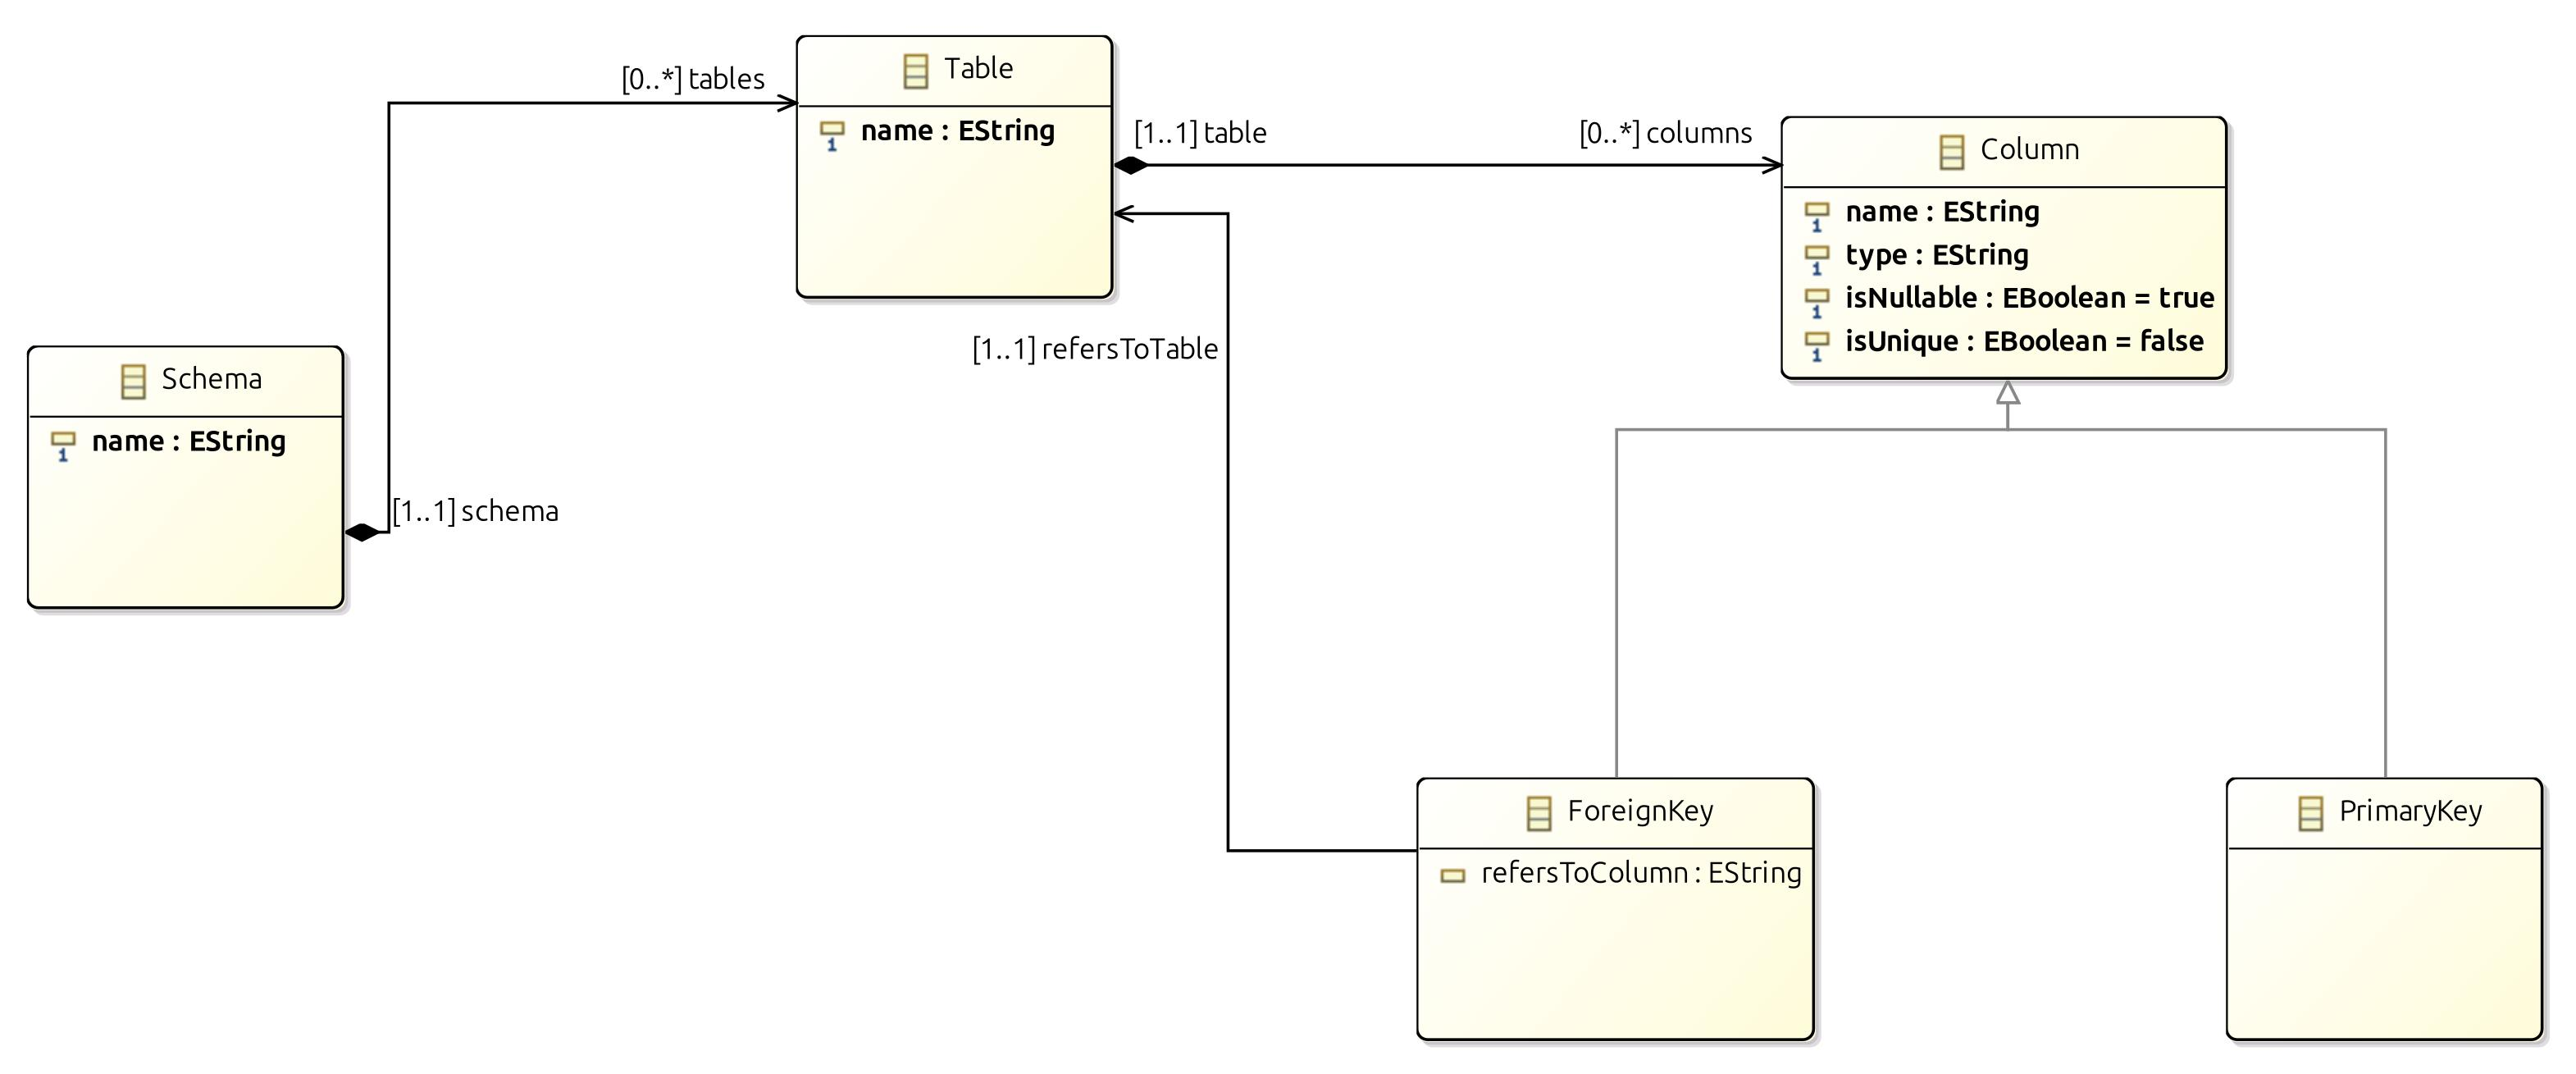
\includegraphics[width=1.0\textwidth]{imgs/relational-metamodel.png}
            \caption{Relational Metamodel}
        \label{figure4}
    \end{figure}
\end{center}

Note that the generalization of Column into Primary Key and Foreign Key is an incomplete and disjoint generalization. In terms of implementation, three attributes were added to Column:

\begin{itemize}

    \item \textbf{isPrimaryKey}: (boolean - EBoolean), which defaults to False and indicates whether this column is a primary key in the corresponding table;
 
    \item \textbf{isForeignKey}: (boolean - EBoolean), which defaults to False and indicates whether this column is a foreign key in the corresponding table;
    
    \item \textbf{refersToColumn}: (string - EString), which defaults to Null and represents the name of the referenced table if this column is a foreign key.
    
\end{itemize}

Multiplicities do not need to be explicitly defined in the metamodel, as they are expressed by the existence of foreign keys between tables or by adding new tables, which will be ensured by the model-to-model transformation discussed in later sections.

\section{Metamodel Constraints}

In this section, we explored the constraints and validations of the metamodels. This process involved applying various integrity constraints and invariants to ensure that the generated models adhere to the defined rules. The metamodels were subjected to various tests that checked each of the programmed constraints. We used the Object Constraint Language (OCL) within the Ecore framework to express these constraints, providing a mechanism for validating the integrity of our inputs.

\subsection{Constraints}

To maintain data integrity throughout the modeling process, we implemented the following OCL constraints:

\begin{itemize}

    \item \textbf{C1}: The model/schema must contain entities/tables with unique, not-empty names;

    \item \textbf{C2}: All entities/tables must have attributes/columns with unique, not-empty names;
    
    \item \textbf{C3}: All entities/tables must have an identifier/primary key;
    
    \item \textbf{C4}: The lower multiplicity must be less than or equal to the upper bound, and both values must be non-negative;
    
    \item \textbf{C5}: The primary key must be unique and not null;
    
    \item \textbf{C6}: Columns in tables that are foreign keys must refer to an existing table in the system, other than itself;

    \item \textbf{C7}: No schema, table or column name can be an SQL Reserved Word;

    \item \textbf{C8}: The column type must a valid SQL data type;

    \item \textbf{C9}: The column referenced by a foreign key must be UNIQUE;

    \item \textbf{C10}: The referenced table of a foreign key must have the referenced column;

    \item \textbf{C11}: The column type of a foreign key must be of the same type as the one it references.

\end{itemize}

Constraints C1 to C3 were implemented in both metamodels, while C4 applies only to the ER Metamodel. Constraints C5 to C11 are specific to the Relational Metamodel. The implementation details can be found in the \textbf{er.ecore} and \textbf{relational.ecore} files submitted.

Another restriction considered was that entities, attributes, or relationships, can only be used inside the respective schema. It was thought on this constraint, as it can only be one schema per each XMI file.

These constraints ensure that the models are well-defined and that the relationships between various components are valid, thereby preserving the integrity of the final database structure.

\subsection{Validation}

The validation of the modeling constraints involved encoding various test cases to verify compliance with the metamodels. This step was essential to confirm that the implemented constraints functioned as intended and that the models adhered to the specifications set in the metamodel design.

The project submission includes a tests folder containing various test cases. For instance, the file \textbf{test1-er.xmi} was used as input for the ER metamodel to test Constraint 1 (C1), while \textbf{test5-relational.xmi} served as input for the Relational Metamodel to test Constraint 5 (C5).  In addition to incorporating all the previously explored constraints, the new files also serve to validate the correct functioning of the metamodels when exposed to various ER and Relational system scenarios. These files include examples that cover different types of entities and relationships, allowing for more comprehensive validation. The new files are:

\begin{itemize}

    \item \textbf{entity-\textless{}er, relational\textgreater{}.xmi}: an entity/table with multiple attribute types;
    
    \item \textbf{one-to-one-\textless{}er, relational\textgreater{}.xmi}: two entities with only an ID primary key followed by an one-to-one relationship;
    
    \item \textbf{one-to-many-\textless{}er, relational\textgreater{}.xmi}: two entities with only an ID primary key followed by an one-to-many relationship;
    
    \item \textbf{many-to-many-\textless{}er, relational\textgreater{}.xmi}: two entities with only an ID primary key followed by a many-to-many relationship;
    
    \item \textbf{gym-\textless{}er, relational\textgreater{}.xmi}: a more general example that combines several relationships and entities with multiple attributes, representing a more complex scenario.
    
\end{itemize}

These new files allow for testing and validating the consistency and integration of the metamodels, addressing a wider range of data modeling scenarios, thus ensuring the robustness and flexibility of the system.

Table \ref{constraints-validation} summarizes the expected and obtained results for each test case following validation attempts.

\begin{table}[H]
\begin{tabular}{|c|c|c|c| }
\hline
\textbf{\begin{tabular}[c]{@{}c@{}}Targeted\\Constraint\end{tabular}} & \textbf{Test File}                              & \textbf{\begin{tabular}[c]{@{}c@{}}Expected\\Result\end{tabular}} & \textbf{Obtained Result} \\ \hline
\textit{C1}         & test1-\textless{}er, relational\textgreater{}.xmi   & Fail                     & Fail                     \\ \hline
\textit{C2}         & test2-\textless{}er, relational\textgreater{}.xmi   & Fail                     & Fail                     \\ \hline
\textit{C3}         & test3-\textless{}er, relational\textgreater{}.xmi   & Fail                     & Fail                     \\ \hline
\textit{C4}         & test4-er.xmi                                        & Fail                     & Fail                     \\ \hline
\textit{C5}         & test5-relational.xmi                                & Fail                     & Fail                     \\ \hline
\textit{C6}         & test6-relational.xmi                                & Fail                     & Fail                     \\ \hline
\textit{C7}         & test7-relational.xmi                                & Fail                     & Fail                     \\ \hline
\textit{C8}         & test8-relational.xmi                                & Fail                     & Fail                     \\ \hline
\textit{C9}         & test9-relational.xmi                                & Fail                     & Fail                     \\ \hline
\textit{C10}         & test10-relational.xmi                                & Fail                     & Fail                     \\ \hline
\textit{C11}         & test11-relational.xmi                                & Fail                     & Fail                     \\ \hline
\textit{All}         & gym-\textless{}er, relational\textgreater{}.xmi     & Success                  & Success                  \\ \hline
\end{tabular}
\caption{Validation Results for Metamodel Constraints}
\label{constraints-validation}
\end{table}

Full coverage of all constraints was achieved, ensuring the integrity of the generated ER and Relational metamodels.

\section{Model-to-Model Transformations}

In this section, we explored the transformation process from the Entity-Relationship model to the Relational model. This process involved applying various integrity constraints to ensure that the transformed models adhere to the defined rules\footnote{https://www.geeksforgeeks.org/mapping-from-er-model-to-relational-model/}. We used Atlas Transformation Language (ATL) within the Ecore framework to express these constraints, providing a mechanism for validating the integrity of our transformations.

\subsection{Constraints}

The transformation of an Entity-Relationship model to a Relational model required several steps to ensure that the data and its meaning are not lost in the process. The problem was divided into five essential steps so that the development of the ATL code would cover all the specifications.

\subsubsection{Model to Schema}

The Model is the root element of the ER Model, while the Schema is the main element in Relational systems. Both have an associated \textbf{name}, so the transformation is simple and involves a direct transition: the name of the final Schema is the same as the name of the initial Model.

\subsubsection{Entity to Table}

Within the Model, which is the root element of the ER Model, there are Entities. These are related to the Tables to be added within the Schema in the Relational Model. While the name of the resulting Table is simply the same as the name of the Entity, its attributes become columns, with some additional checks:

\begin{itemize}

    \item the resulting column will have the same name as the attribute;
    
    \item the type of the resulting column is the same as the type of the attribute from the entity;
    
    \item if \textbf{isIdentifier = true}, it means that the column to be added must be a \textbf{Primary Key}. In this case, the column also has \textbf{isNullable = false} and \textbf{isUnique = true} by default;
    
    \item otherwise, the transformation copies the original attribute's characteristics of \textbf{isNullable} and \textbf{isUnique} to the final column.

\end{itemize}

Figure \ref{figure5} illustrates and summarizes the transformation of an Entity between the models studied.

\begin{center}
    \begin{figure}[H]
        \centering
        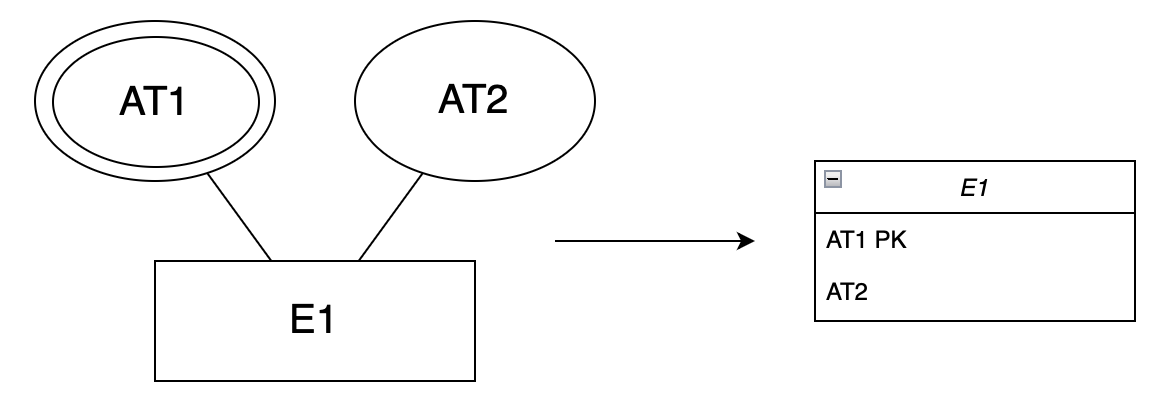
\includegraphics[width=0.8\textwidth]{imgs/entity-transformation.png}
            \caption{Entity to Table Transformation}
        \label{figure5}
    \end{figure}
\end{center}

\subsubsection{One-to-One Relationships}

In the example where there is a relationship between two entities, with each entity being related to the other in equal cardinality and multiplicity, in the Relational Model it is necessary to add a \textbf{Foreign Key} to the table of one of them. This Foreign Key is a new column in that table with the following characteristics:

\begin{itemize}

    \item its name is, for example, the concatenation of the name of the table it relates to with the suffix \textbf{\_id};
    
    \item it must be \textbf{isNullable = false} and \textbf{isUnique = true};
    
    \item \textbf{refersToTable} is the name of the table it relates to;
    
    \item \textbf{refersToColumn} is the name of the column that is the primary key of the related table.

\end{itemize}

Figure \ref{figure6} illustrates the transformation of this type of relationship between entities.

\begin{center}
    \begin{figure}[H]
        \centering
        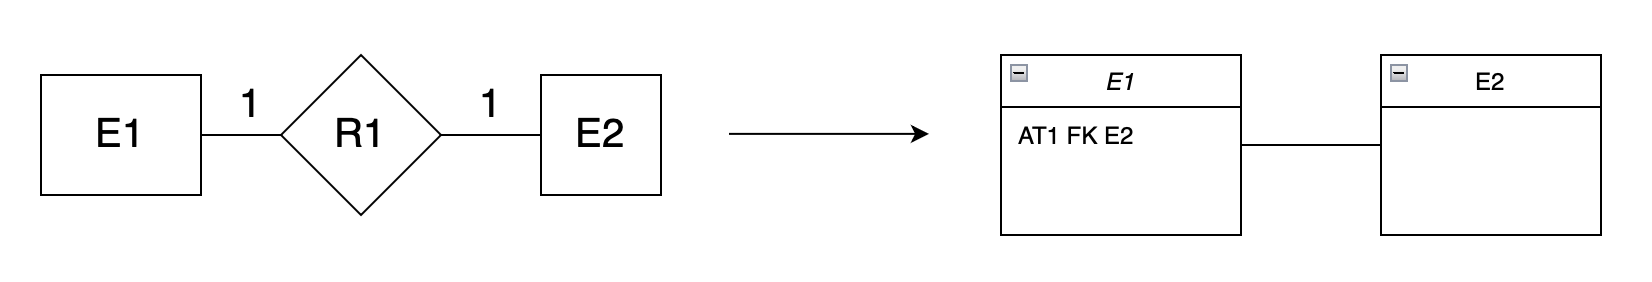
\includegraphics[width=1.0\textwidth]{imgs/one-to-one-transformation.png}
            \caption{One-to-One Relationships Transformation}
        \label{figure6}
    \end{figure}
\end{center}

\subsubsection{One-to-Many Relationships}

In the case of having a relationship between entities with different multiplicities and cardinalities in the system, whether it is because one entity is related to several others, or several entities are related to the same target entity, it is necessary to take an approach similar to the one explained earlier. However, the table chosen to hold the new Foreign Key is not just random: it is the table with the greater multiplicity that will have a new column to associate with the other table.

Figure \ref{figure7} illustrates this transformation.

\begin{center}
    \begin{figure}[H]
        \centering
        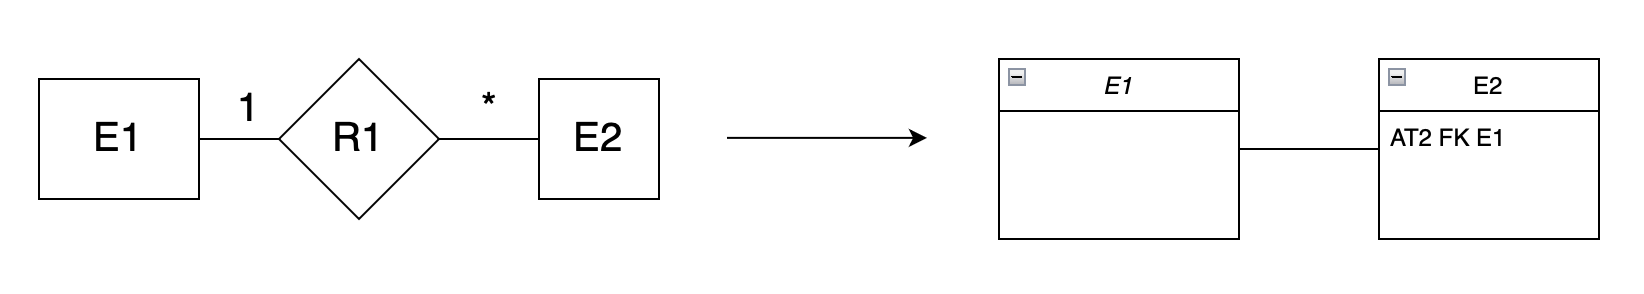
\includegraphics[width=1.0\textwidth]{imgs/one-to-many-transformation.png}
            \caption{One-to-Many Relationships Transformation}
        \label{figure7}
    \end{figure}
\end{center}

\subsubsection{Many-to-Many Relationships}

Unlike other types of relationships, there would be a loss of information from the system if only one foreign key were added to one of the tables, or if a pair of foreign keys were added mutually. The solution to accommodate this in the Relational model is that the relationship results in a new table in the final Schema, with the following characteristics:

\begin{itemize}

    \item the name of the new table is the name of the relationship;
    
    \item the table has two foreign key columns, both with \textbf{isNullable = false} and \textbf{isUnique = true} by default;
    
    \item each column points to the respective source entity:
    
        \begin{itemize}
    
            \item \textbf{refersToTable}: the name of the table to be referenced;
            
            \item \textbf{refersToColumn}: the name of the column that is the primary key of the referenced table;
    
        \end{itemize}
    
\end{itemize}

Figure \ref{figure8} illustrates what happens to the system in this type of transformation.

\begin{center}
    \begin{figure}[H]
        \centering
        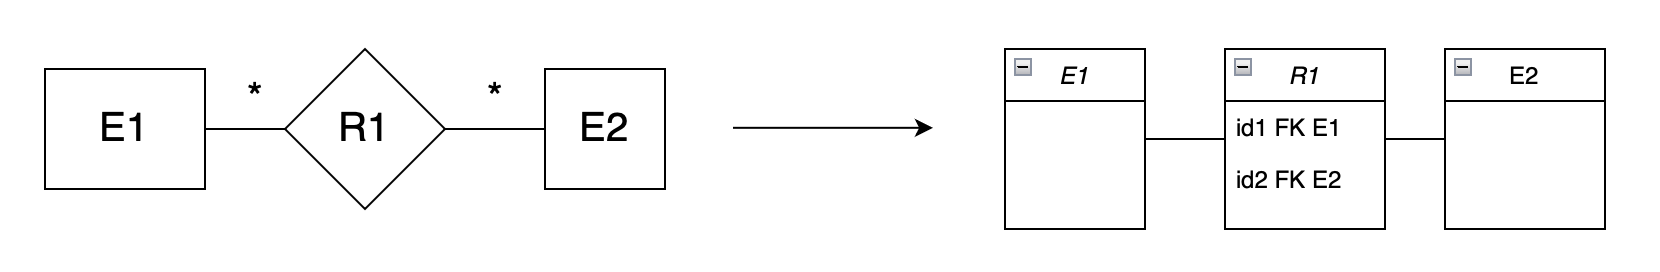
\includegraphics[width=1.0\textwidth]{imgs/many-to-many-transformation.png}
            \caption{Many-to-Many Relationships Transformation}
        \label{figure8}
    \end{figure}
\end{center}

The file attached in the project submission, \textbf{er2relational.atl}, contains the ATL code that is capable of performing the transformations between models.

\subsection{Validation}

To validate the transformation between models, the successful tests from the previous step were used to ensure that all constraints and contents were maintained between systems. After obtaining the target Relational Model from each of the files that characterize the source ER Models using the ATL code, the Relational Metamodel was used to validate each of the output models. Table \ref{transformations-validation} summarizes the results obtained.

\begin{table}[H]
\centering
\begin{tabularx}{\textwidth}{|>{\centering\arraybackslash}X|>{\centering\arraybackslash}X|>{\centering\arraybackslash}p{3.5cm}|}
\hline
\textbf{Input ER File} & \textbf{Output Relational File} & \textbf{Valid Output ?} \\ \hline
gym-er.xmi & gym-relational.xmi & Yes \\ \hline
\end{tabularx}
\caption{Validation of Model-to-Model transformations}
\label{transformations-validation}
\end{table}

In this way, we demonstrate that the models generated by this transformation are in accordance with the intended outcome and comply with all the constraints imposed in the previous section.

\section{Model-to-Text Transformations}

In this section, we explored the transformation process from the Relational model to the final SQL code. This process involved applying standard rules\footnote{https://www.geeksforgeeks.org/relational-model-in-dbms/} across the previously defined schema. We used Model Transformation Language (MTL) with Accelelo within the Ecore framework to express these rules, providing a mechanism for creating and validating the integrity of our final transformation.

\subsection{Transformation}

Since the transformation from the ER model to the relational model has already handled the mapping of multiplicities into new columns as foreign keys and/or new tables within the same schema, formalized each table with its respective attributes and primary keys, and validated each output using the Relational Metamodel, the starting point for this part of the transformation was appropriately structured and verified.

For logical reasons, the final SQL writing was carried out in three main stages:

\subsubsection{Schema to SQL}

The first part of writing executable and valid SQL code is the declaration and selection of the schema. The schema name depends solely on the name specified in the corresponding model.

\begin{lstlisting}
CREATE SCHEMA IF NOT EXISTS GymSchema;
\end{lstlisting}

\subsubsection{SQL Constraints}

In SQL systems, it's essential that previous declarations in the schema do not conflict with the new table declarations we will subsequently add to the file. For this reason, it is important to include statements like \textbf{DROP TABLE IF EXISTS} for each table. After declaring the schema and before adding the tables from the previous schema, we dropped each one using a simple loop.

\begin{lstlisting}
DROP TABLE IF EXISTS Gym;
DROP TABLE IF EXISTS Equipment;
DROP TABLE IF EXISTS Customer;
\end{lstlisting}

\subsubsection{Table to SQL}

For each table, its attributes were declared, considering characteristics such as:

\begin{itemize}

    \item name;
    
    \item type, which is mapped to VARCHAR, INT, or FLOAT types;
    
    \item isNullable, which is mapped to the NOT NULL constraint;
    
    \item isUnique, which is mapped to the UNIQUE constraint;
    
    \item refersToTable: the name of the table to be referenced, in the case of a foreign key;
    
    \item refersToColumn: the name of the column that is the primary key of the referenced table, important in the case of a foreign key.

\end{itemize}

\begin{lstlisting}
CREATE TABLE Equipment (
	id INT NOT NULL UNIQUE,
	name VARCHAR,
	min_weight FLOAT,
	max_weight FLOAT,
	gym_id INT NOT NULL UNIQUE,
	
	PRIMARY KEY (id),
	FOREIGN KEY (gym_id) REFERENCES Gym (id)
);
\end{lstlisting}

The complete transformation of the \textbf{gym-relational.xmi} model is available in Annex \ref{Annex1}. The file attached in the project submission, \textbf{relational2sql.mtl}, contains the MTL code that is capable of performing these transformations.

\subsection{Validation}

The output validation consisted of verifying the SQL generated in the previous step, ensuring it adheres to the language standards overall. The SQL code was considered valid if:

\begin{itemize}

    \item no syntactic errors were present;
    
    \item no semantic errors were present;
    
    \item it could be executed with a database engine like PostgreSQL\footnote{https://www.postgresql.org},  SQLite3\footnote{https://www.sqlite.org} or MySQL\footnote{https://www.mysql.com};
    
\end{itemize}

We used the Online SQL Validator\footnote{https://aiven.io/tools/sql-syntax-checker} to check the SQL integrity. Table \ref{sql-validation} summarizes the results obtained.

\begin{table}[H]
\centering
\begin{tabularx}{\textwidth}{|>{\centering\arraybackslash}X|>{\centering\arraybackslash}X|>{\centering\arraybackslash}p{3.5cm}|}
\hline
\textbf{Input Relational File} & \textbf{Output SQL File} & \textbf{Valid SQL ?} \\ \hline
gym-relational.xmi & gym-relational.sql & Yes \\ \hline
\end{tabularx}
\caption{Validation of Model-to-Text transformations}
\label{sql-validation}
\end{table}

The data shows that this functionality enabled the creation of a pipeline with two validated and sequential transformations, capable of transforming an ER model into its corresponding SQL perspective.

\section{Conclusion}

In this project, we explored and implemented key techniques within Model-Driven Software Engineering to automate application development on low-code platforms. 

We began with Modeling Domain Analysis, gaining a deep understanding of the domain to ensure our models reflected real-world concepts accurately. This analysis guided the subsequent design of the modeling language. We then focused on Modeling Language Design, contributing to the development of both ER and Relational models that captured the structure and relationships of the data effectively.

In the Development of Integrity Constraints, we ensured that the models adhered to necessary rules to maintain data consistency and enforce business logic. The project also involved the Creation and Testing of Models, Metamodels, and Transformations, where we built and validated both the models and their corresponding metamodels, ensuring accurate transformations between them.

Through these efforts, we built a foundation for understanding the core components of the modeling process, ensuring the integrity and validity of the models while enabling automation on low-code platforms.

\section{Contributions}

The group members have contributed equally for the project's development. As a result, it was given the same grade in percentage, so that its sum is 100\%, as shown on the list below:

\begin{itemize}

    \item \textbf{Fábio Sá}: 25\%;

    \item \textbf{Filipe Fonseca}: 25\%;
    
    \item \textbf{Lourenço Gonçalves}: 25\%;
    
    \item \textbf{Pedro Ferreira}: 25\%.
    
\end{itemize}

In qualitative terms, all the group members have contributed in the whole project process. In other words, every group member has helped with:

\begin{itemize}

    \item Modeling Domain Analysis;

    \item Modeling Language Design, contributing the development of ER and Relational models;

    \item Development of integrity constraints for the models;
    
    \item Models, Metamodels and Transformations creation and testing;
    
    \item Writing the report.
    
\end{itemize}

\newpage
\bibliographystyle{apalike}
\bibliography{references}

\newpage
\appendix 

\section{Gym Example SQL} \label{Annex1}

\begin{lstlisting}[language=SQL]
CREATE SCHEMA IF NOT EXISTS GymSchema;

DROP TABLE IF EXISTS Gym;
DROP TABLE IF EXISTS Equipment;
DROP TABLE IF EXISTS Customer;

CREATE TABLE Equipment (
	id INT NOT NULL UNIQUE,
	name VARCHAR,
	min_weight FLOAT,
	max_weight FLOAT,
	gym_id INT NOT NULL UNIQUE,
	
	PRIMARY KEY (id),
	FOREIGN KEY (gym_id) REFERENCES Gym (id)
);

CREATE TABLE Gym (
	id INT NOT NULL UNIQUE,
	name VARCHAR NOT NULL UNIQUE,
	address VARCHAR NOT NULL,
	tax_id INT NOT NULL UNIQUE,
	
	PRIMARY KEY (id)
);

CREATE TABLE Customer (
	id INT NOT NULL UNIQUE,
	name VARCHAR NOT NULL,
	address VARCHAR NOT NULL,
	age INT NOT NULL,
	tax_id INT NOT NULL UNIQUE,
	
	PRIMARY KEY (id)
);
\end{lstlisting}

\end{document}
